\documentclass[semifinal]{cpecmu}

%% This is a sample document demonstrating how to use the CPECMU
%% project template. If you are having trouble, see "cpecmu.pdf" for
%% documentation.

\projectNo{45}%
\acadyear{2020}

\titleTH{เว็บบล๊อกสำหรับผู้ที่สนใจเกี่ยวกับกาแฟ}
\titleEN{Coffee Blog}

\author{นางสาวศศิรัตน์ มณีเจียร}{Sasirat Maneejian}{600610778}

\cpeadvisor{navadon}
\cpecommittee{santi}
\cpecommittee{lachana}
%% Some possible packages to include:
\usepackage[final]{graphicx} % for including graphics

%% Add bookmarks and hyperlinks in the document.
\usepackage[colorlinks=true,allcolors=Blue4,citecolor=red,linktoc=all]{hyperref}

%% Needed just by this example, but maybe not by most reports
\usepackage{afterpage} % for outputting
\usepackage{pdflscape} % for landscape figures and tables. 

%% Some other useful packages. Look these up to find out how to use
%% them.
% \usepackage{natbib}    % for author-year citation styles
% \usepackage{txfonts}
% \usepackage{appendix}  % for appendices on a per-chapter basis
% \usepackage{xtab}      % for tables that go over multiple pages
% \usepackage{subfigure} % for subfigures within a figure
% \usepackage{pstricks,pdftricks} % for access to special PostScript and PDF commands
% \usepackage{nomencl}   % if you have a list of abbreviations

%% if you're having problems with overfull boxes, you may need to increase
%% the tolerance to 9999
% \tolerance=9999

\bibliographystyle{plain}
% \bibliographystyle{IEEEbib}

% \renewcommand{\topfraction}{0.85}
% \renewcommand{\textfraction}{0.1}
% \renewcommand{\floatpagefraction}{0.75}

%% Example for glossary entry
%% Need to use glossary option
%% See glossaries package for complete documentation.
\ifglossary
  \newglossaryentry{lorem ipsum}{
    name=lorem ipsum,
    description={derived from Latin dolorem ipsum, translated as ``pain itself''}
  }
\fi

%% Uncomment this command to preview only specified LaTeX file(s)
%% imported with \include command below.
%% Any other file imported via \include but not specified here will not
%% be previewed.
%% Useful if your report is large, as you might not want to build
%% the entire file when editing a certain part of your report.
% \includeonly{chapters/intro,chapters/background}

\begin{document}
\maketitle
\makesignature

\ifproject
\begin{abstractTH}
เว็บบล็อคสำหรับผู้ที่สนใจเกี่ยวกับกาแฟ เป็นเว็บไซต์ที่จัดทำขึ้นเพื่อรวบรวมบทความเกี่ยวกับกาแฟ เพื่อให้ผู้ที่สนใจเกี่ยวกับกาแฟมีพื้นที่ในการแลกเปลี่ยนความรู้ และนำเสนอกาแฟในรูปแบบของตนเอง เช่น เจ้าของร้านกาแฟ เกษตรกรผู้ที่ปลูกกาแฟ ผู้ที่ทำการคั่วกาแฟ หรือผู้ที่สนใจในด้านกาแฟทั้งผู้ที่เริ่มต้นและผู้ที่สนใจแบบจริงจัง และเพื่อทำให้มี Web blog ที่มีความเฉพาะเจาะจงเกี่ยวกับกาแฟ 
\end{abstractTH}

\begin{abstract}
Coffee blog, a website created for users who interested in coffee so that they can place to exchange knowledge and their own style of coffee, such as coffee owner, coffee roaster, or those interested in the coffee both beginner and amateur. 
\end{abstract}

\iffalse
\begin{dedication}
This document is dedicated to all Chiang Mai University students.

Dedication page is optional.
\end{dedication}
\fi % \iffalse

\begin{acknowledgments}
Your acknowledgments go here. Make sure it sits inside the
\texttt{acknowledgment} environment.

\acksign{2020}{5}{25}
\end{acknowledgments}%
\fi % \ifproject

\contentspage

\ifproject
\figurelistpage

\tablelistpage
\fi % \ifproject

% \abbrlist % this page is optional

% \symlist % this page is optional

% \preface % this section is optional


\pagestyle{empty}\cleardoublepage
\normalspacing \setcounter{page}{1} \pagenumbering{arabic} \pagestyle{cpecmu}

\chapter{\ifcpe บทนำ\else Introduction\fi}

\section{\ifcpe ที่มาของโครงงาน\else Project rationale\fi}

\section{\ifcpe วัตถุประสงค์ของโครงงาน\else Objectives\fi}
\begin{enumerate}
    \item
\end{enumerate}

\section{\ifcpe ขอบเขตของโครงงาน\else Project scope\fi}

\subsection{\ifcpe ขอบเขตด้านฮาร์ดแวร์\else Hardware scope\fi}

\subsection{\ifcpe ขอบเขตด้านซอฟต์แวร์\else Software scope\fi}

\section{\ifcpe ประโยชน์ที่ได้รับ\else Expected outcomes\fi}

\section{\ifcpe เทคโนโลยีและเครื่องมือที่ใช้\else Technology and tools\fi}

\subsection{\ifcpe เทคโนโลยีด้านฮาร์ดแวร์\else Hardware technology\fi}

\subsection{\ifcpe เทคโนโลยีด้านซอฟต์แวร์\else Software technology\fi}

\section{\ifcpe แผนการดำเนินงาน\else Project plan\fi}

\begin{plan}{6}{2020}{2}{2021}
    \planitem{7}{2020}{8}{2020}{ศึกษาค้นคว้า}
    \planitem{8}{2020}{1}{2021}{ชิล}
    \planitem{2}{2021}{2}{2021}{เผา}
    \planitem{12}{2019}{1}{2022}{ทดสอบ}
\end{plan}

\section{\ifcpe บทบาทและความรับผิดชอบ\else Roles and responsibilities\fi}
อธิบายว่าในการทำงาน นศ. มีการกำหนดบทบาทและแบ่งหน้าที่งานอย่างไรในการทำงาน จำเป็นต้องใช้ความรู้ใดในการทำงานบ้าง

\section{\ifcpe%
ผลกระทบด้านสังคม สุขภาพ ความปลอดภัย กฎหมาย และวัฒนธรรม
\else%
Impacts of this project on society, health, safety, legal, and cultural issues
\fi}

แนวทางและโยชน์ในการประยุกต์ใช้งานโครงงานกับงานในด้านอื่นๆ รวมถึงผลกระทบในด้านสังคมและสิ่งแวดล้อมจากการใช้ความรู้ทางวิศวกรรมที่ได้

\chapter{\ifcpe ทฤษฎีที่เกี่ยวข้อง\else Background Knowledge and Theory\fi}

การทำโครงงาน เริ่มต้นด้วยการศึกษาค้นคว้า ทฤษฎีที่เกี่ยวข้อง หรือ งานวิจัย/โครงงาน ที่เคยมีผู้นำเสนอไว้แล้ว ซึ่งเนื้อหาในบทนี้ก็จะเกี่ยวกับการอธิบายถึงสิ่งที่เกี่ยวข้องกับโครงงาน เพื่อให้ผู้อ่านเข้าใจเนื้อหาในบทถัดๆ ไปได้ง่ายขึ้น

\section{ความสำคัญของกาแฟ}
กาแฟเป็นพืชเศรษฐกิจสำคัญประเภทหนึ่งซึ่ง เป็นสินค้าที่มีโอกาสและศักยภาพสูงในการทำตลาด โดยได้รับการจัดอันดับว่าเป็นพิชเศรษฐกิจที่มีมูลค่าสูง และนำไแแปรรูปให้มีมูลค่าสูงมากไปอีก โดยในประเทศไทยเป็นผู้ส่งออกกาแฟสำเร็จรูปอยู่ในอันดับที่ 11 ของโลกในปี พ.ศ. 2562 และในประเทศไทยคนส่วนดื่มกาแฟเผื่อบ่งบอกรสนิยมส่วนตัวด้วย โดยมีตัวเลขบ่งบอกว่าคนไทยดื่มกาแฟคนละ 300 แก้วต่อปี ซึ่งมีผลต่ออัตราการขยายตัวของตลาดกาแฟในประเทศไทย การมีร้านค่าเฟ่ที่ขายกาแฟที่มากขึ้นในประเทศไทยที่มีเอกลักษณ์และความสวยงามทำให้ผู้คนมีความสนใจที่จะไปร้านมากขึ้นและทำให้หลายๆคนได้ลองดื่มกาแฟแบบใหม่ๆ และผลเนื่องมาจาก Covid-19 ผู้คนมีความต้องการกาแฟสูงขึ้น ทำให้ผู้ประกอบการร้านกาแฟต้องทำแบบเดลิเวรี่ ซึ่งทำให้กาแฟสำเร็จรูปนั้นมีโอกาสในการส่งออกมากขึ้น

\section{Spacialty coffee}
Specialty Coffee คือ กาแฟพิเศษ ที่วัดกันตั้งแต่เมล็ดกาแฟจนถึง Process ทุกอย่างครับ เมล็ดกาแฟที่เป็น Specialty Coffee ต้องเป็นเมล็ดที่ชงออกมาแล้วผ่านกระบวนการคัด คั่ว บด กลั่น ชง จนได้กาแฟที่มีรสชาติดี ได้รับการรับรองว่ามีคุณภาพจากนักชิมที่มีความเชี่ยวชาญ ที่เรียกว่า Cupper หรือ Q – Grader โดยมีการทดสอบว่าในเรื่องกระบวนการผลิตเมล็ดกาแฟ การทดสอบคุณภาพ การทดสอบกลิ่นและรสชาติ และต้องได้คะแนน 80 คะแนนขึ้นไป ถึงจะเรียกว่า Specialty Coffee ได้ \cite{special}

\section{Coffee Taster's Flavor Wheel}
วงล้อกลิ่นและรสชาติกาแฟ เป็นเครื่องมือที่มีประโยชน์มากๆสำหรับนักชิมกาแฟ ในการวิเคราะห์และอธิบายกลิ่นและรสชาติกาแฟ เพราะบางครั้งมันก็เป็นอะไรที่ยากสำหรับมือใหม่ เนื่องจากการชิมกาแฟนั้น มีหลากหลายขั้นตอนที่ต้องทำเวลา และควบคุมอุณหภูมิ การจะวิเคราะห์รสชาติและกลิ่นนั้นอาจอยู่ภายใต้การจิบเร็วๆ เพียงไม่กี่ครั้ง แต่ ประโยชน์ที่แท้จริงของวงล้อสีนี้ คือเป็น Guideline สำคัญ ให้กับทั้งคนดื่ม และคนชงกาแฟ คุยกันรู้เรื่อง, ผมก็เลยแยกแบ่งเป็นกลุ่มหมวดต่างๆ 9 หมวด เพื่อให้มองเห็นชัด และเข้าใจได้ง่ายขึ้น \cite{wheel}

ซึ่งภายในเว็บไซต์ที่ทำจะให้การวิเคราะห์นี้ในการรีวิวกาแฟ เพื่อให้ผู้ใช้ได้มีความสนุกมากขึ้นในชิมกาแฟต่างๆ แบ่งปันรสชาติ และแสดงความคิดเห็นเกี่ยวกับรสชาติของกาแฟที่ตนเองได้ชิมให้ผู้ที่เข้ามาอ่านเห็นภาพและมีความน่าสนใจมากขึ้น

\section{การพัฒนาซอฟต์แวร์}
\subsection{React}
React เป็น JavaScript Library ที่ Facebook เป็นผู้พัฒนาโดยเปิดเป็น opem source โดยมี 3 concept หลักคือ Component, state และ Props โดยข้อดีของ React ก็คือมีเครื่อมือทำงานด้วยเยอะซึ่งเป็นประโยชน์ต่อการพัฒนามาก

\subsection{Next.js}
Next.js เป็น framwork ที่ใช้สำหรับสร้างเว็บ โดยใช้ react เพื่อให้กระบวนการง่ายขึ้น ซึ่งข้อดีของ Next.js คือ มี route ให้ และใช้ง่านกับ css แบบ Module หรือ CSS-in-JS


\section{\ifcpe%
ความรู้ตามหลักสูตรซึ่งถูกนำมาใช้หรือบูรณาการในโครงงาน
\else%
ISNE knowledge used, applied, or integrated in this project
\fi
}

อธิบายถึงความรู้ และแนวทางการนำความรู้ต่างๆ ที่ได้เรียนตามหลักสูตร ซึ่งถูกนำมาใช้ในโครงงาน

\section{\ifcpe%
ความรู้นอกหลักสูตรซึ่งถูกนำมาใช้หรือบูรณาการในโครงงาน
\else%
Extracurricular knowledge used, applied, or integrated in this project
\fi
}

อธิบายถึงความรู้ต่างๆ ที่เรียนรู้ด้วยตนเอง และแนวทางการนำความรู้เหล่านั้นมาใช้ในโครงงาน

\chapter{\ifproject%
\ifcpe โครงสร้างและขั้นตอนการทำงาน\else Project Structure and Methodology\fi
\else%
\ifcpe โครงสร้างของโครงงาน\else Project Structure\fi
\fi
}

ในบทนี้จะกล่าวถึงหลักการทำงาน และการออกแบบระบบของการเขียนบทความและการรีวิวกาแฟ

\makeatletter

% \renewcommand\section{\@startsection {section}{1}{\z@}%
%                                    {13.5ex \@plus -1ex \@minus -.2ex}%
%                                    {2.3ex \@plus.2ex}%
%                                    {\normalfont\large\bfseries}}

\makeatother
%\vspace{2ex}
% \titleformat{\section}{\normalfont\bfseries}{\thesection}{1em}{}
% \titlespacing*{\section}{0pt}{10ex}{0pt}

\section{การใช้งานของระบบ}
Usecase diagram ซึ่งเป็นการแสดงภาพรวมของการใช้งานของระบบ โดยจะแบ่งผู้ใช้งานเป็นสองกลุ่มคือ กลุ่มผู้เขียนบทความและรีวิว และกลุ่มผู้อ่านบทความ ซึ่งผู้ใช้ทั้งสองฝั่งจะใช้งานผ่านเว็บไซต์ Coffee blog 

\begin{figure}[h]
\begin{center}
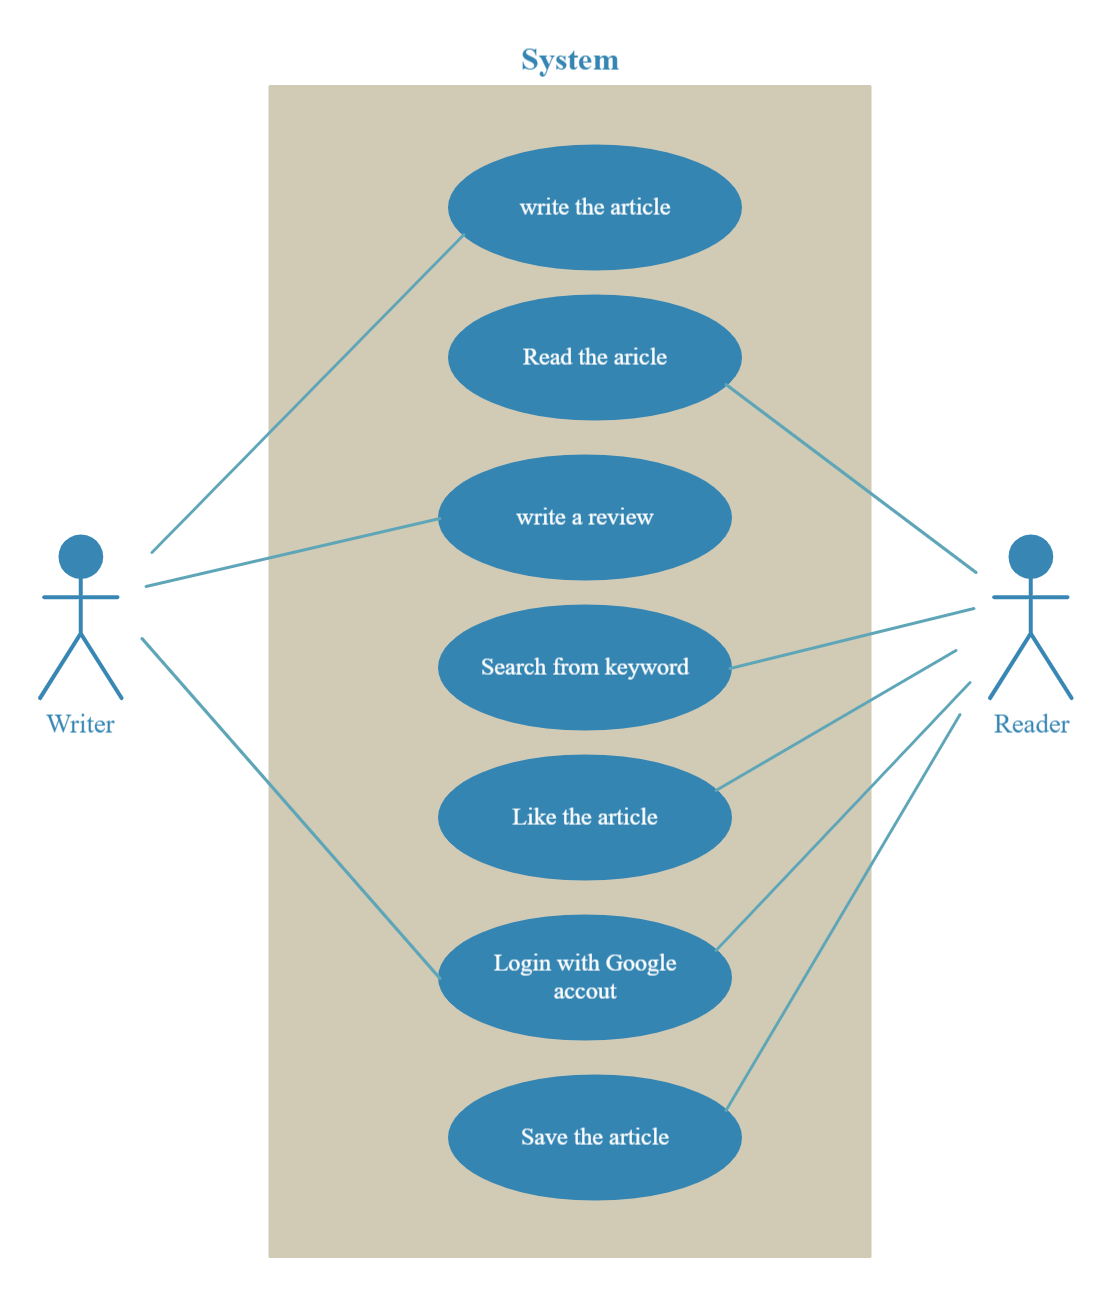
\includegraphics[width=6cm, height=8cm]{usecase-diagram.jpg}
\end{center}
\caption[Usecase diagram]{usecase diagram ของระบบ}
\end{figure}

การใช้งานของระบบจะมีการทำงานดังตัวอย่างต่อไปนี้ \\ 
Use case 1 \\ 
Usecase Title : การเขียนบทความ\\
Primary Actor : ผู้เขียนบทความ\\
Stakeholder Actor : ผู้อ่านบทความ\\
Main Flow : ผู้ใช้ทั้งสองฝั่งเข้าสู่ระบบด้วย Google account ผู้ที่เขียนบทความเข้าไปเขียนบทความในหน้าบทความ และกดโพสต์บทความเพื่อทำการสร้างบทความ และเลือก tag สำหรับบทความเพื่อให้ผู้ที่เข้ามาอ่านสามารถค้นหาบทความได้ง่ายขึ้น\\
Exceptional Flow : เมื่อเขียนบทความเสร็จ ผู้อ่านจะสามารถเข้ามาอ่านได้ ยอดการเข้าอ่านบทความจะเพิ่มขึ้น\\ \\
Use case 2 \\
Usecase Title : การอ่านบทความ\\
Primary Actor : ผู้อ่านบทความ\\
 Stakeholder Actor : ผู้เขียนบทความ\\
Main Flow : ผู้ใช้ทั้งสองฝั่งเข้าสู่ระบบด้วย Google account ในหน้าแรกผู้ใช้สามารถค้นหา keyword ที่ต้องการเข้าไปอ่านได้ ถ้าผู้ใช้ชอบบทความที่เข้าไปอ่านผู้ใช้สามารถ like บทความ และ save ไว้อ่านทีหลังได้\\
 Exceptional Flow : เมื่อกด save บทความผู้ใช้จะสามารถเข้าไปดูบทความที่ save ได้\\ \\
Use case 3\\
Usecase Title : การเขียนรีวิว\\
Primary Actor : ผู้เขียนรีวิว\\
 Stakeholder Actor : ผู้อ่านรีวิว\\
Main Flow : ผู้ที่ต้องการเขียนรีวิว จะถ่ายรูปกาแฟ หรือถุงกาแฟที่ตนเองต้องการรีวิว และอัพโหลดไปที่เว็บไซต์ เขียนรายระเอียดเกี่ยวกับกาแฟ และเลือกสีที่ต้องการ \\
 Exceptional Flow : เมื่อเขียนรีวิวเสร็จ ผลลัพธ์ที่ได้จะได้เป็นหน้าแสดงผล เช่นกราฟ และสรุปของสี ที่เกี่ยวกับกาแฟ\\

 \section{โครงสร้างของระบบ}
 โดยภาพรวมของระบบจะเป็นดังภาพ ซึ่งในส่วนของผู้ใช้ หรือ client จะใช้ React Next.js ในการพัฒนา และมีตัวกลางในการติดต่อเรียกใช้ข้อมูลระหว่าง server กับ client คือ GraphQL และในส่วนของ server จะใช้ Nodejs ในการพัฒนา ฐานข้อมูล จะมีสองส่วน คือ Elasticsearch จะทำในส่วนของการเก็บข้อมูลที่ใช้ในการ search และ MongoDB ที่จะเก็บข้อมูลต่างๆ
\begin{figure}[h]
\begin{center}
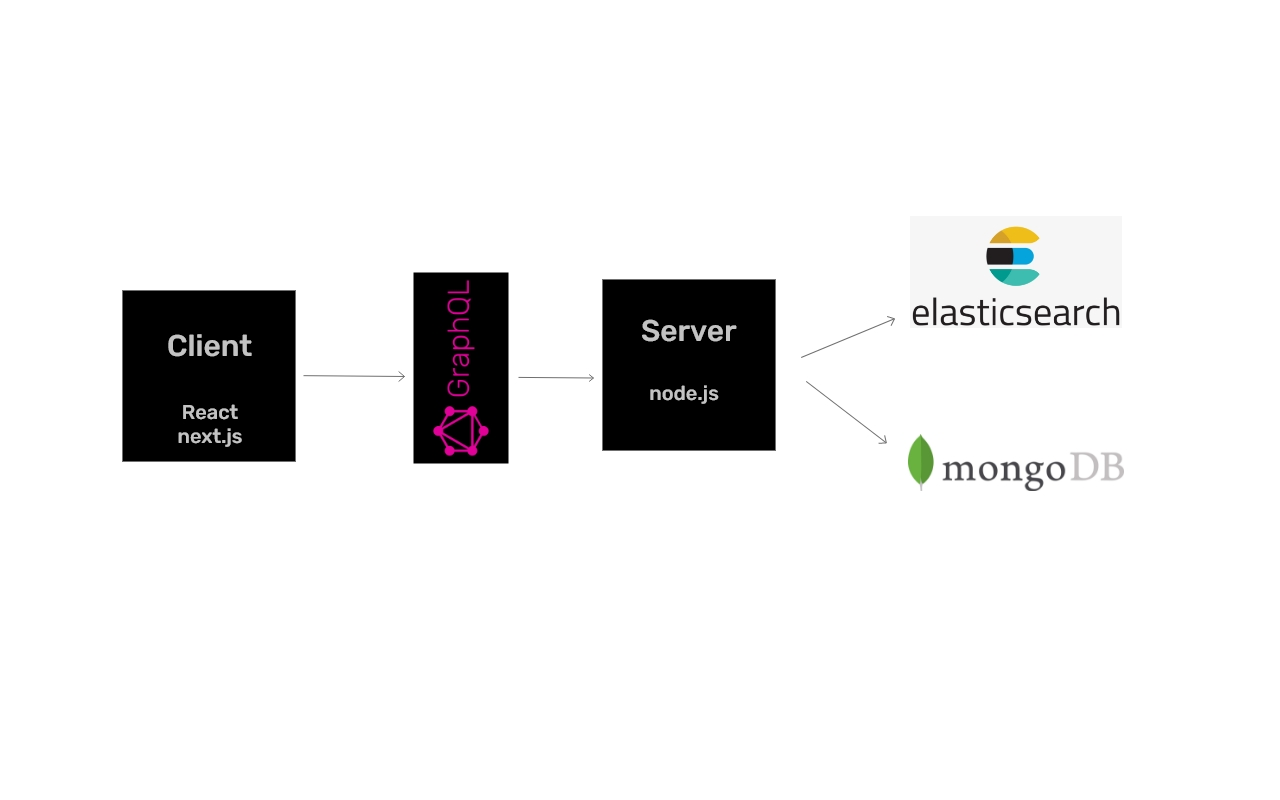
\includegraphics[width=10cm, height=8cm]{database.jpg}
\end{center}
\caption[Application Model]{แผนผังการทำงานของระบบ}
\end{figure}
หลักการทำงานของระบบ
\begin{enumerate}
  \item ผู้ใช้สามารถเข้าเว็บไซต์ได้จากสมาร์ทโฟน แท็บเล็ต หรือคอมพิวเตอร์
  \item เมื่อผู้ใช้ต้องการค้นหาบทความจะเรียกของมูลมาจาก elasticsearch โดยใช้ graphql เป็นตัวกลางในการเรียกใช้ข้อมูล
  \item เมื่อผู้ใช้ต้องการเขียนบทความหรือเขียนรีวิว ข้อมูลจะอัพเดตและเก็บไว้ใน MongoDB 
  \item การทำงานของผู้ใช้ทั้งหมดจะสามารถใช้งานบนเว็บไซต์ทั้งหมด
\end{enumerate}
สาเหตุที่ทำเว็บไซต์เพื่อให้ผู้ใช้สามารถเข้าถึงได้ในอุปกรณ์ต่างๆ และมีความง่ายต่อการพัฒนา

\chapter{\ifproject%
\ifcpe การทดลองและผลลัพธ์\else Experimentation and Results\fi
\else%
\ifcpe การประเมินระบบ\else System Evaluation\fi
\fi}

ในบทนี้จะทดสอบเกี่ยวกับการทำงานในฟังก์ชันหลักๆ

\ifproject
% \chapter{\ifcpe บทสรุปและข้อเสนอแนะ\else Conclusions and Discussion\fi}

\section{\ifcpe สรุปผล\else Conclusions\fi}

นศ. ควรสรุปถึงข้อจำกัดของระบบในด้านต่างๆ ที่ระบบมีในเนื้อหาส่วนนี้ด้วย

\section{\ifcpe ปัญหาที่พบและแนวทางการแก้ไข\else Challenges\fi}

ในการทำโครงงานนี้ พบว่าเกิดปัญหาหลักๆ ดังนี้

\section{\ifcpe%
ข้อเสนอแนะและแนวทางการพัฒนาต่อ
\else%
Suggestions and further improvements
\fi
}

ข้อเสนอแนะเพื่อพัฒนาโครงงานนี้ต่อไป มีดังนี้

\fi

\bibliography{sampleReport}

% \ifproject
% \appendix
% \chapter{The first appendix}

Text for the first appendix goes here.

\section{Appendix section}

Text for a section in the first appendix goes here.

\verb+test ทดสอบฟอนต์ teletype ภาษาไทย+

\texttt{test ทดสอบฟอนต์ teletype ภาษาไทย}

\chapter{\ifcpe คู่มือการใช้งานระบบ\else Manual\fi}

Manual goes here.


% %% Display glossary (optional) -- need glossary option.
% \ifglossary\glossarypage\fi

%% Display index (optional) -- need idx option.
% \ifindex\indexpage\fi

% \begin{biosketch}
% \begin{center}
%   
\includegraphics[width=1.5in]{mugshot.jpg}
% \end{center}
% Your biosketch goes here. Make sure it sits inside
% the \texttt{biosketch} environment.
% \end{biosketch}
% \fi % \ifproject
\end{document}
